\chapter{Design Approach}
\section{Proposed System}
A transaction server is a specialized type of server that manages the operations of software-based transactions or transaction processing. It manages application and database transactions on a network or Internet, within a distributed computing environment.
\par
A transaction server may also be referred to as a transaction processing system (TPS) or as a part of one composite TPS solution. A transaction server primarily enables transactions to be processed within distributed computing applications. Typically, a transaction server is a combination of hardware, software and network components that altogether ensures completion of each transaction. A transaction server works when an application or application server requests for a specific data object residing on a database or database server on the network or Internet. The transaction server acts as an intermediary server that can ensure that the application or user receives the requested data from the database or the completion of that transaction.
\par
The transaction server is also the name of a Microsoft Server (Viper) or Microsoft transaction server (MTS), which provides similar functionality. It provides transaction processing services on the COM/DCOM based software components.
\par
Distributed computing is a computing concept that, in its most general sense, refers to multiple computer systems working on a single problem. In distributed computing, a single problem is divided into many parts, and each part is solved by different computers. As long as the computers are networked, they can communicate with each other to solve the problem. If done properly, the computers perform like a single entity.
\par
The ultimate goal of distributed computing is to maximize performance by connecting users and IT resources in a cost-effective, transparent and reliable manner. It also ensures fault tolerance and enables resource accessibility in the event that one of the components fails.
\par
This first started with the use of data entry terminals on mainframe computers, then moved into minicomputers and is now possible in personal computers and client-server architecture with more tiers.
\par
A distributed computing architecture consists of a number of client machines with very lightweight software agents installed with one or more dedicated distributed computing management servers. The agents running on the client machines usually detect when the machine is idle and send a notification to the management server that the machine is not in use and available for a processing job. The agents then requests an application package. When the client machine receives this application package from the management server to process, it runs the application software when it has free CPU cycles and sends the result back to the management server. When the user returns and requires the resources again, the management server returns the resources was using to perform different tasks in the user's absence.
\section{Architecture}
\begin{figure}[ht]
\centering
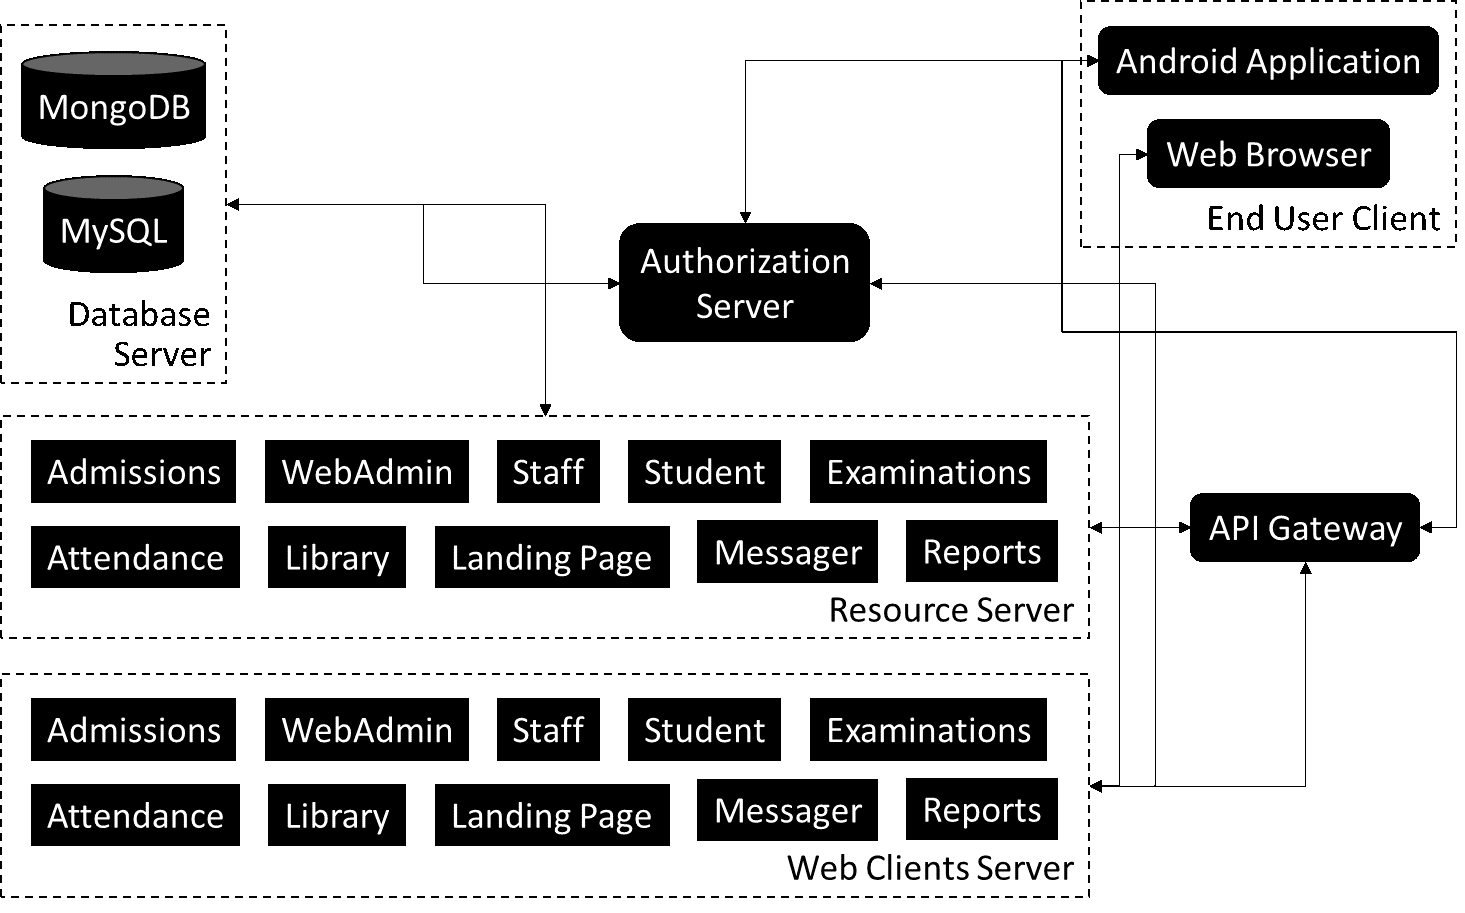
\includegraphics[width=35em]{figures/figure6.png}
\caption{OAuth 2.0 Flow}
\end{figure}